% !TEX root = ../../main.tex
\newpage

\section{Umgang mit \protect\LaTeX{}}%{{{
\label{sec:umgang}
\subsection{Seitenaufbau}%{{{
\label{sec:seit-aufbau}
Der Seitenaufbau wird vollständig in der Präambel (siehe meta/preamble.tex) definiert. Das macht den Umgang mit \gls{latex} für eine wissenschaftliche Arbeit so attraktiv. Grundsätzlich erlaubt es der Workflow von \gls{latex}, sich vollständig auf den Inhalt zu konzentrieren und so wenig wie nötig sich mit \glqq Design\grqq\ aufzuhalten.

Die Dokumentenklasse gibt an, um was für ein Dokument es sich handelt\footcite[Vgl. ][S. 9]{oetiker_not_2018}. Dieses Dokument nutzt die Dokumentenklasse \glqq scrartcl\grqq\footcite[S. 51]{kohm_koma_2019}\ aus dem bekannten Paket \hologo{KOMAScript}. Diese hat sich für unseren Einsatzzweck bereits vielfach bewährt und sollte somit ein sicheres Mittel sein.
Die Klasse wird mit einigen Parametern geladen, wie zum Beispiel \glqq 12pt\grqq, welches die Schriftgröße auf 12 festlegt. Erwähnenswert ist die Funktion \glqq overfullrule\grqq, denn Sie kann zum Schluss dabei helfen, sogenannte \glqq overfull hbox Error\grqq\ zu finden. Diese werden zwar im log protokolliert, das finden gestaltet sich allerdings manchmal schwierig. Mit der Option werden an die entsprechende Stellen dann schwarze Kästchen gedruckt, was die Suche extrem vereinfacht. Typischerweise zeigt die Warnung auf, dass
in der entsprechenden Zeile zu viel dargestellt wird und der Seitenrand überschrieben wird. Dies ist oft damit verbunden, das \LaTeX{}\ nicht wusste, wie es das Wort richtig trennen soll. Diese Wörter lassen sich dann selbst definieren, so dass \LaTeX{}\ die Silbentrennung beim nächsten Durchlauf korrekt durchführen kann.
Zusätzlich ist die Option \glqq draft\grqq\ bei größeren Dokumenten hilfreich, denn es verarbeitet nicht alle Informationen und spart dadurch Zeit beim kompilieren. Diese Vorlage wird z. B. aus diesen Gründen im ersten Durchlauf ebenfalls nur als \glqq draft\grqq-Variante kompiliert, da wir praktisch nur die Output-Dateien brauchen, die weiter als Input für \hologo{biber}, makeglossaries und xindy dienen.

Das Paket geometry setzt das Seitenlayout auf die gewünschten Einheiten.

Wichtig zum problemfreien Einsatz der KOMA-Klasse ist, dass ihr das Paket \glqq fancyhdr\grqq\ meidet, da es dafür eigene Befehle und Werkzeuge gibt. Ich verweise hier auf den ~\ref{lst:our-heafoo}.

\lstinputlisting[firstline=23,lastline=46,float=htpb,caption=Der relevante Code für Header und Footer,label=lst:our-heafoo]{meta/preamble.tex}

Im Text stehen euch dann weitere Befehle zur Verfügung. In main.tex wird z. B. einige Male die Paginierung umgestellt. Mit dem Befehlt \textbackslash pagenumberingstil lassen sich die in der Tabelle~\ref{tab:pgnumb} gezeigten Stile einstellen.

\begin{table}[htpb]
  \centering
  \begin{tabular}{|c|c|}
    \hline
    arabic & arabische Zahlen \\ \hline
    roman & kleine, römische Zahlen \\ \hline
    Roman & große, römische Zahlen \\ \hline
    alph & kleine Buchstaben \\ \hline
    Alph & große Buchstaben \\ \hline
  \end{tabular}
  \caption{Die verschiedenen Stile der Paginierung}
  \label{tab:pgnumb}
\end{table}

Sollten mal Angaben von Abständen oder ähnlichem erfordert sein, so versteht \LaTeX{}\ die Einheiten \emph{mm}, \emph{cm}, \emph{in} (Inch), \emph{pt} (Point = $\frac{1}{72} in$), \emph{em} (Proportional zur Zeichenbreite), und \emph{ex} (Proportional zur Zeichenhöhe)\footcite[Vgl. ][S. 5]{riedel_latex_2011}.

Weitere Informationen über den Umgang mit \hologo{KOMAScript} erhaltet ihr in dem ausgezeichnetem Handbuch des Pakets, welches wenigstens für gezielte Fragen zwingend konsultiert werden sollte. Außerdem gibt es noch die Möglichkeit auf der \href{https://komascript.de/}{Website des Paketes \protect\hologo{KOMAScript}} auf ein Forum sowie ein FAQ zurückzugreifen.

Diese Vorlage nutzt die Vorgaben des \gls{fb} Wirtschaftswissenschaften, welcher durchaus von anderen \glspl{fb} abweichen kann. Die entsprechenden Änderungen sollten allerdings relativ einfach umzusetzen sein. Gerne addiere ich an spätere Stelle hier entsprechende Vorlagen neben dieser.%}}}
\subsection{Textformatierung}%{{{
\label{sec:textformat}
Da dies hier den Rahmen sprengen würde, möchte ich auf eine sehr gute, kostenfreie Einführung verweisen, welche Kompakt und gut verständlich die Feinheiten von \gls{latex} erklärt. Über sechs Kapitel wird dann angefangen bei der grundsätzlichen Struktur eines Dokumentes bis hin dazu, wie man grundlegende Funktionen von \gls{latex} umschreibt, und das alles auf 153 Seiten, kostenlos.\footcite{oetiker_not_2018}

\begin{table}[htbp]
  \resizebox{\textwidth}{!}{% gently resize our table to fit the page
  \centering
    \begin{tabular}{|l|l|l|}
    \hline
    Befehl & Effekt & Anmerkung \\ \hline
    \textbackslash emph\{Befehl\} & \emph{Befehl} & Bevorzugt, wählt automatisch zwischen textbf und textit \\ \hline
    \textbackslash textbf\{Befehl\} & \textbf{Befehl} &  \\ \hline
    \textbackslash textit\{Befehl\} & \textit{Befehl} &  \\ \hline
    \textbackslash textsl\{Befehl\} & \textsl{Befehl} &  \\ \hline
    \textbackslash underline\{Befehl\} & \underline{Befehl} & Sollte angepasst werden, da das Standardverhalten \\ %\cline{1-2}
    & & womöglich ein unerwartetes Ergebnis produziert \\ \hline
    \end{tabular}%
  }
  \caption{Grundlegende Textformatierung}
  \label{tab:textformat}
\end{table}

Einige grundlegende Befehle findet man aber bereits in Tabelle~\ref{tab:textformat}.
%}}}
\subsection{Allgemeiner Umgang mit Zahlen}%{{{
\label{sec:allgzahl}
Mit der Schreibumgebung \textbackslash num des Paketes siunitx ist es möglich, Zahlen gut leserlich im Text darzustellen, wenn es noch nicht um die Darstellung von reiner Mathematik geht. Beispielsweise in einem Satz: Zum Zeitpunkt der Erstellung hat der Bau des neuen Berliner Flughafens BER \num[group-separator={.}]{4645889099}\EUR\ gekostet.
\begin{lstlisting}[float=htpb,caption=Darstellung von Zahlen in \protect\LaTeX{},label=lst:zahlen]
Zum Zeitpunkt der Erstellung hat der Bau des neuen Berliner Flughafens BER \num[group-separator={.}]{4645889099}\EUR\ gekostet.
\end{lstlisting}

Das Paket kann durchaus noch vieles mehr, so wie zum Beispiel die korrekte Darstellung von Maßeinheiten:
\si{\kilo\gram\metre\per\square\second} \\
\si{\gram\per\cubic\centi\metre}
\\
\si{\square\volt\cubic\lumen\per\farad} \\
\si{\metre\squared\per\gray\cubic\lux}

\begin{lstlisting}[float=htpb,caption=Darstellungen von Einheiten mit siunitx,label=lst:einheiten]
\si{\kilo\gram\metre\per\square\second} \\
\si{\gram\per\cubic\centi\metre}
\\
\si{\square\volt\cubic\lumen\per\farad} \\
\si{\metre\squared\per\gray\cubic\lux}
\end{lstlisting}

Ein Blick ins Handbuch wird daher definitiv empfohlen.
%}}}
\subsection{Mathematische Schreibumgebung}%{{{
\label{sec:math-umg}
Wenn man Code zwischen zwei Dollar Zeichen \$ \dots\ \$ schreibt, schreibt man in dem mathematischen Modus. Alles darin wird interpretiert und durch entsprechende Symbole ersetzt. Das Ergebnis spricht für sich.

$ SEW\footnote{Summe der Endwerte} (RF\footnote{Rückflüsse}) = \sum_{t=1}^{n} [ ( E_{t} - A_{t}) \times (1+i)\ ^{N-t}] $

$ SEW(RF) = 5\times1,1^{5}+10\times1,1^{4}+15\times1,1^{3}+10\times1,1^{2}+30\times1,1^{1}+35 = 122,76$

$ i_{m} = \sqrt[N]{\dfrac{SEW(RF)}{BW(IA)}} -1$

$ i_{m} = \sqrt[6]{\dfrac{122,76}{50}} -1 = 0,1615 \approx 16,15\%$

$ SEW(RF) = 186,72 $

$ i_{m} = 0,1097 \approx 10,97\%$

Der Code hierfür sieht wie folgt aus:
\begin{lstlisting}[float=htpb,caption=Darstellungen von mathematischen Formeln,label=lst:inlinemath]
$ SEW\footnote{Summe der Endwerte} (RF\footnote{Rückflüsse}) = \sum_{t=1}^{n} [ ( E_{t} - A_{t}) \times (1+i)\ ^{N-t}] $

$ SEW(RF) = 5\times1,1^{5}+10\times1,1^{4}+15\times1,1^{3}+10\times1,1^{2}+30\times1,1^{1}+35 = 122,76$

$ i_{m} = \sqrt[N]{\dfrac{SEW(RF)}{BW(IA)}} -1$

$ i_{m} = \sqrt[6]{\dfrac{122,76}{50}} -1 = 0,1615 \approx 16,15\%$

$ SEW(RF) = 186,72 $

$ i_{m} = 0,1097 \approx 10,97\%$
\end{lstlisting}

Grundsätzlich unterstützt \gls{latex} aber noch eine weitere Methode, mathematische Sequenzen darzustellen, z. B. das sogenannte \glqq Displayed math\grqq.

\[
  \varphi = \frac{1 + \sqrt{5}}{2} = 1.618 \ldots
\]

Code:

\begin{lstlisting}[float=htpb,caption=Darstellungen von Mathe mit der \glqq displayed math\grqq-Methode,label=lst:dspmath]
\[
  \varphi = \frac{1 + \sqrt{5}}{2} = 1.618 \ldots
\]
\end{lstlisting}

Man unterscheidet beide Methoden in 1) \emph{Inline math} (vergleiche~\ref{lst:inlinemath}) und 2) \emph{Displayed math} (vergleiche~\ref{lst:dspmath}).\footcite[Vgl. ][S. 276]{kottwitz_latex_2015} \emph{Inline math} eignet sich, um Formeln im Text einzufügen, \emph{Displayed math} präsentiert die Formel in einer eigenen Zeile. Bei letzterem ist auch die Nummerierung der Zeilen möglich.

\gls{latex} bietet darüber hinaus noch sehr viel mehr Einstellmöglichkeiten, um Formeln besser darzustellen. Dazu lohnt sich ein Blick in geeignete Fachliteratur, wie zum Beispiel auch Grätzers \glqq More Math into \LaTeX{}\grqq\footcite{gratzer_more_2016}.
%}}}
\subsection{Tabellen}%{{{
\label{sec:tables}
Tabellen lassen sich natürlich auch in \gls{latex} schreiben, allerdings gestaltet sich das auf den ersten Blick etwas umständlich. Als Beispiel dafür, die recht simple, Tabelle~\ref{tab:tab1}.
\begin{table}[htbp]
\resizebox{\textwidth}{!}{%
\begin{tabular}{|l|l|l|l|l|l|l|}
\hline
t & 0 & 1 & 2 & 3 & 4 & 5 \\ \hline
lfd. EZÜ & 262.500 & 352.450 & 455.395 & 572.871 & 706.628 & 858.656 \\ \hline
zstl. ZÜ &  & 89.950 & 192.895 & 310.371 & 444.128 & 596.156 \\ \hline
Barwerte & -550.000 & 84.065 & 168.482 & 253.355 & 338.823 & 425.051 \\ \hline
kumulierter Barwert & 719.776 &  &  &  &  &  \\ \hline
\end{tabular}
}
\caption{Eine einfache Tabelle}
\label{tab:tab1}
\end{table}

Der dazugehörige Code:
\begin{lstlisting}[float=htpb,caption=Darstellungen einer Tabelle in \protect\LaTeX{},label=lst:bsptabelle]
\begin{table}[htbp]
\begin{tabular}{|l|l|l|l|l|l|l|}
\hline
t & 0 & 1 & 2 & 3 & 4 & 5 \\ \hline
lfd. EZÜ & 262.500 & 352.450 & 455.395 & 572.871 & 706.628 & 858.656 \\ \hline
zstl. ZÜ &  & 89.950 & 192.895 & 310.371 & 444.128 & 596.156 \\ \hline
Barwerte & -550.000 & 84.065 & 168.482 & 253.355 & 338.823 & 425.051 \\ \hline
kumulierter Barwert & 719.776 &  &  &  &  &  \\ \hline
\end{tabular}
\caption{Eine einfache Tabelle}
\label{tab:tab1}
\end{table}
\end{lstlisting}

Je nach gewünschtem Stil kann eine Tabelle noch sehr stark verändert werden. Dies schaut man am besten ebenfalls in geeigneter Literatur nach, da es hier den Rahmen sprengen würde.

Ein genereller Tipp aber zum Thema Tabellen: nutzt ein externes Tool. Viele Editoren bringen Tools mit, um Tabellen einfacher zu erstellen. Ich finde folgende Website sehr gut \href{https://tablesgenerator.com}{https://tablesgenerator.com}.
%}}}
\subsection{Grafiken}%{{{
\label{sec:graphics}
Grafiken werden von \LaTeX{}\ dahin gesetzt, wo sie am besten hinpassen. Anhand von zwei beispielhaften Grafiken demonstrieren wir also, wie der freie Wille entscheidet. Da dieser sich im Laufe der Erstellung der Thesis immer wieder ändert, empfiehlt es sich, sich während des Schreibens des eigentlichen Textes sich nicht weiter mit der Platzierung von \glqq Floats\grqq\ aufzuhalten.

\begin{figure}[h!]
  \centering
     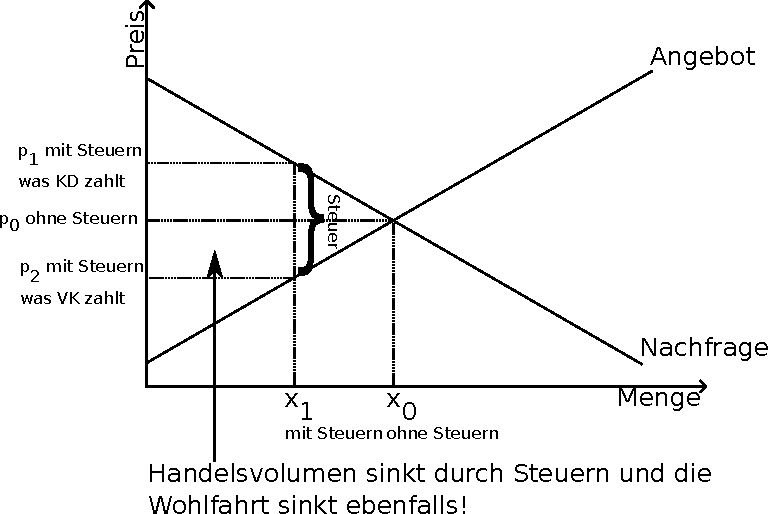
\includegraphics[]{ProdKonsRentemitSteuern.pdf}
     \caption{Die Besteuerung eines Marktes}
     \label{fig:bild}
\end{figure}

.

Die Abbildung~\ref{fig:bild} wurde mit dem Parameter \glqq h!\grqq\ (vgl. ~\ref{lst:float_h}) aufgerufen. Für \LaTeX{}\ heißt dass, das Bild an Ort und stelle abzulegen.%~\ref{} i need to include all other listings in floats

\begin{lstlisting}[float=htpb,caption=Einbindung einer Grafik so nah wie möglich am Text,label=lst:float_h]
  \begin{figure}[h!]
    \centering
       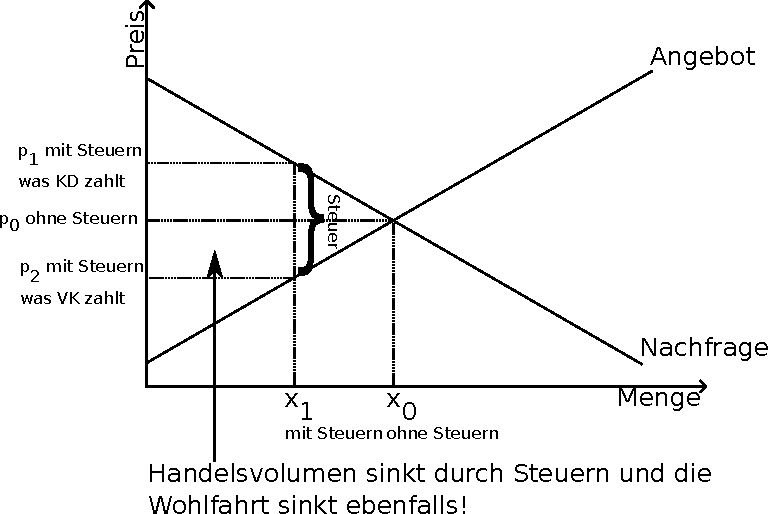
\includegraphics[]{ProdKonsRentemitSteuern.pdf}
    \caption{Die Besteuerung eines Marktes}
    \label{fig:bild}
  \end{figure}
\end{lstlisting}

Die zweite Grafik, Abbildung~\ref{fig:bild2}, soll die interne Logik verdeutlichen. Dieses mal hat \LaTeX{}\ mehr Freiheiten durch die Parameter \glqq htbp\grqq\ (vgl. ~\ref{lst:float_htbp}).

\begin{figure}[htbp]
  \centering
     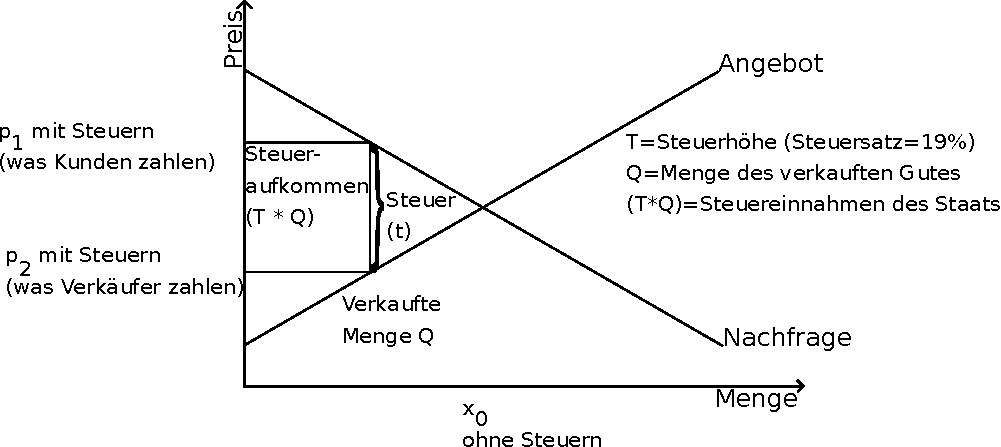
\includegraphics[width=1\linewidth]{PMSteuer.pdf}
  \caption{Steueraufkommen}
  \label{fig:bild2}
\end{figure}

Hier schreibe ich noch mal etwas Text hin, der keinen Sinn ergibt, wenigstens nicht zwangsläufig, immerhin soll \gls{latex} rund um meine beiden Beispielbilder etwas Text zu verarbeiten haben, damit der Leser/Anwender es später selbst etwas einfacher hat, sich das Konzept vor Augen zu führen. Kommentiert einfach etwas Text raus, ändert die Größe der Grafiken oder die angegebenen Parameter und ihr solltet ein Bild davon bekommen, was \LaTeX{}\ sich bei der Sache denkt.

Zusätzlich erhält dieser Block einen neuen Absatz. Das Thema Bienensterben ist ein ernstes Thema auf welches man an dieser Stelle aufmerksam machen kann, da sie sehr wichtig für das Ökosystem unseres Planeten sind.

\begin{lstlisting}[float=htpb,caption=Automatische Einbindung einer Grafik,label=lst:float_htbp]
\begin{figure}[htbp]
  \centering
  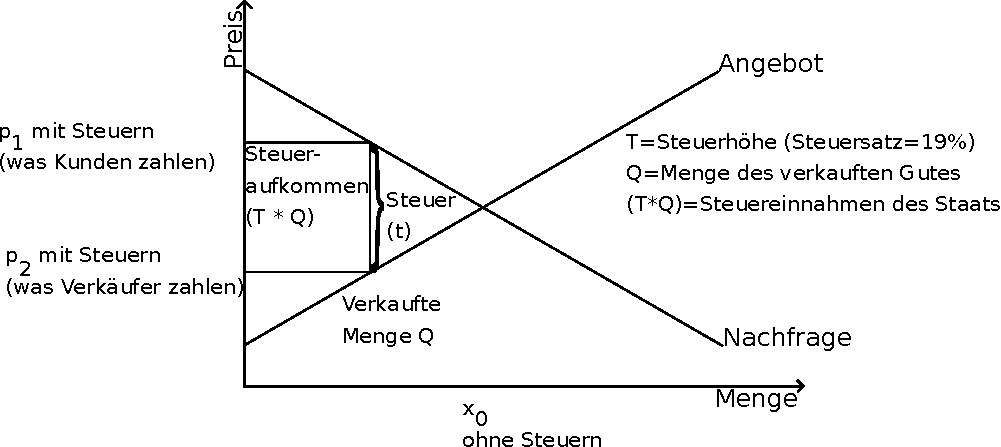
\includegraphics[width=1\linewidth]{PMSteuer.pdf}
  \caption{Steueraufkommen}
  \label{fig:bild2}
\end{figure}
\end{lstlisting}
%}}}
\subsection{Grafiken mit TikZ}%{{{
\label{sec:tikzgraph}
\LaTeX{} bietet eine eigene \emph{Vektorzeichenumgebung} an: \glqq TikZ\grqq! Selbst habe ich es noch nicht verwendet, allerdings passt die Art sehr gut in das Gesamtdokument. Darüber hinaus folgt die Syntax einer relativ einfachen Logik, was also durchaus bei kleineren Grafiken Zeit sparen kann.

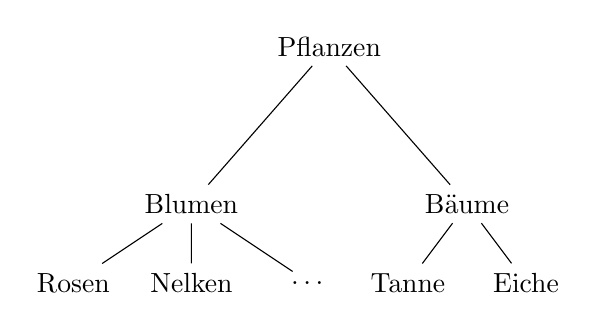
\begin{tikzpicture}
  [level 1/.style={sibling distance=35mm,
    level distance=20mm},
    level 2/.style={sibling distance=15mm,
    level distance=10mm}]
  \node {Pflanzen}
    child {node {Blumen}
    child {node {Rosen}}
    child {node {Nelken}}
    child {node {\ldots}}
  }
    child {node {Bäume}
    child {node {Tanne}}
    child {node {Eiche}}
  };
\end{tikzpicture}

Folgendes Beispiel stammt von Christine Römer\footcite{dtk17.1:roemer:tikz} und wurde in \glqq Die \TeX{}nische Komödie\grqq\ veröffentlicht. Die Zeitschrift wird von \glspl{dante} herausgegebenen.
%}}}
\subsection{Fußnoten}%{{{
\label{sec:footn}
Fußnoten werden über den Befehl \textbackslash footnote gesetzt und automatisch im Footer fortlaufend Nummeriert aufgeführt.\footnote{\href{https://de.wikibooks.org/wiki/LaTeX-W\%C3\%B6rterbuch:_footnote}{Mehr auf Wikibooks}}
\begin{lstlisting}[float=htpb,caption=Das Setzen von Fußnoten mit \protect\LaTeX{},label=lst:footnotes]
Fußnoten werden über den Befehl \footnote{Meine erste Fußnote} gesetzt und automatisch im Footer fortlaufend Nummeriert aufgeführt.\footnote{\href{https://de.wikibooks.org/wiki/LaTeX-W\%C3\%B6rterbuch:_footnote}{Mehr auf Wikibooks}}
\end{lstlisting}
%}}}
\subsection{Code}%{{{
\label{sec:code}
Code wird am Besten, genau wie eine Grafik (siehe Kapitel~\ref{sec:graphics}), in einer eigenen Umgebung eingefügt. Erstens kümmert sich \gls{latex} nun selbstständig um die Platzierung, zweitens können wir dem \glqq Float\grqq\ ein Label verpassen, dass wir dann referenzieren können.

\begin{lstlisting}[language=Ruby,float=htpb,caption=Beispielcode,label=bspcode]
#!/usr/bin/env ruby

listofstrings = ARGV
puts listofstrings.sort.uniq
\end{lstlisting}

Der Code hierfür:
\begin{lstlisting}[language=Ruby,float=htpb,caption=Darstellung eines beliebigen Codes in der Sprache ruby,label=lst:ruby]
\textbackslash begin{lstlisting}[float=htpb,caption=Beispielcode,label=bspcode]
#!/usr/bin/env ruby

listofstrings = ARGV
puts listofstrings.sort.uniq
\textbackslash end{lstlisting}
\end{lstlisting}
Es ist möglich, die dargestellte Sprache über den Parameter language, hier Ruby, anzupassen. Für das Beispiel musste ich aber die begin/end-Umgebung aufbrechen, da ansonsten der Compiler durcheinander kommt. \gls{latex}-Code in einer Ruby-Umgebung scheint nicht gut mit dem Paket zu funktionieren.

Sollte man diese Funktion gar nicht gebrauchen, kann man die letzten Zeilen in der Präambel dafür kommentieren, damit die Pakete nicht zwingend geladen werden müssen. Das sollte die Performance steigern und mögliche Kompatibilitätsschwierigkeiten, sofern vorhanden, zuvorkommen.

Erwähnenswert ist, dass listings offensichtlich Probleme hat, wenn in einem Kommentar ein ' steht. Woran das liegt, kann ich bisher nicht einschätzen. Memo an mich selbst: Es gibt alternativ zu dem Paket listing auch noch das Paket minted. Eventuell funktioniert das besser?
%}}}
\subsection{Zitieren}%{{{
Zitation scheint mit eines der heikeligsten Angelegenheiten in einer Thesis zu sein. Muss es aber gar nicht. Denn hier kommt \hologo{BibTeX}.

Dieses Sektion wurde außerdem mit Hilfe der üblichen Internetadressen (vorwiegend \href{https://tex.stackexchange.com/}{TeX - LaTeX Stack Exchange}), aber auch einem Blick ins Handbuch von biblatex \footcite{lehman_biblatex_2017}, vorzugsweise in der englischen Originalfassung \footcite{kime_biblatex_2019}, da das Paket ständig überarbeitet wird und somit neue Optionen dazukommen, oder bekannte Optionen ersetzt werden, geschrieben.

Es sei zu erwähnen, das biber\footcite[][]{kime_biber_2019} ebenfalls ein eigenes Handbuch hat, dass weiterhelfen kann!

\begin{lstlisting}[float=htpb,caption=Das Setzen von Zitaten in \protect\LaTeX{},label=lst:cites]
Es sei zu erwähnen, das biber\footcite[][]{kime_biber_2019} ebenfalls ein eigenes Handbuch hat, dass weiterhelfen kann!
\end{lstlisting}
Relevanter Code:
\lstinputlisting[firstline=139,lastline=160,float=htpb,caption=Relevanter Code für biblatex,label=lst:our-bib]{meta/preamble.tex}

In Tabelle ~\ref{tab:bib-style} will ich eine kleine Übersicht über die verfügbaren Stile gestalten. Wir benötigen den \gls{apa}-Stil.

\begin{table}[htbp]
\centering
\resizebox{\textwidth}{!}{%
\begin{tabular}{l|l|l|}
\hline
\multicolumn{1}{|l|}{\textbf{Option}} & \textbf{Wert} & \textbf{\begin{tabular}[c]{@{}l@{}}nennenswerter \\ Effekt\end{tabular}} \\ \hline
\multicolumn{1}{|l|}{autocite} & footnote & Setzt eine Fußnote \\ \hline
 & cite & setzt den Verweis direkt im Text \\ \cline{2-3}
 & parencite & setzt den Verweis im Text in Klammern \\ \hline
\multicolumn{1}{|l|}{style} & numeric & \begin{tabular}[c]{@{}l@{}}Literatur wird numerisch im Verzeichnis\\ aufgeführt\end{tabular} \\ \hline
 & numeric-comp & \begin{tabular}[c]{@{}l@{}}Wie oben, aber mehrerer aufeinanderfolgende\\ Werke werden zusammengefasst\end{tabular} \\ \cline{2-3}
 & alphabetic & \begin{tabular}[c]{@{}l@{}}Erstellt ein Kürzel des Autors und hängt eine\\ fortlaufende Ziffer dran (numeric Verhalten)\end{tabular} \\ \cline{2-3}
 & authoryear & Sortiert nach Autor und Jahr \\ \cline{2-3}
 & authoryear-comp & siehe oben \\ \cline{2-3}
 & authoryear-ibid & setzt ein ebenda, bzw. ebd. \\ \cline{2-3}
 & authoryear-icomp & vereint -comp und -ibid \\ \cline{2-3}
 & authortitle & Sortiert nach Autor und Jahr \\ \cline{2-3}
 & authortitle-comp & siehe oben \\ \cline{2-3}
 & authortitle-ibid &  \\ \cline{2-3}
 & authortitle-icomp &  \\ \cline{2-3}
 & authortite-terse & \begin{tabular}[c]{@{}l@{}}Lässt den Titel aus, wenn der Author nur ein\\ Werk in unserem Literaturverzeichnis hat\end{tabular} \\ \cline{2-3}
 & authortitle-tcomp & Vereint -comp und -terse \\ \cline{2-3}
 & authortitle-ticomp & -comp, -ibid, -terse \\ \cline{2-3}
 & apa & ziemliche vollständiger \gls{apa} Stil der 6ten Edition \\ \cline{2-3}
\end{tabular}%
}
\caption{Einige Optionen zu verwendbaren Zitationsstilen}
\label{tab:bib-style}
\end{table}

Die Idee hinter \hologo{BibTeX}\ ist, dass man die Werke einmalig in einer Datenbank erfasst und von dort aus mit einem zugewiesenem \glqq citekey\grqq\ referenziert. Die Erstellung und Verwaltung einer Datenbank ist z. B. über \href{https://www.zotero.org/}{Zotero}\ (Quelloffen), \href{https://www.jabref.org/}{JabRef}\ (Quelloffen) und \href{https://www.citavi.com/}{Citavi}\ (Closed Source) möglich. Da es sich aber, wie bei \LaTeX{}\ üblich um eine einfache Textdatei handelt, kann man die Datenbank auch selbst
schreiben. Das ist vor allem bei kürzeren Werken eine Alternative, wo man nur mit wenigen Quellen arbeiten muss.
Mir hat bei der Verwendung Zotero gut geholfen. Auch hier empfiehlt sich ein Einarbeiten in das Programm, da es doch sehr viele Möglichkeiten zur Verwaltung der genutzten Literatur bietet.

Das hier ist ein Testzitat für einen Aufsatz in einem Sammelwerk\footcite[][]{billen_kundenbindung_2005}, damit wir den genutzten Stil austesten können.

Es ist ebenfalls möglich, ein Zitat im Text in Klammern zu setzen, so wie es z. B. in der Informatik üblicher ist. Dafür ein weiteres Beispielzitat: Lamport \parencite[Siehe][]{lamport_latex_1994} hat das von Don Knuth \parencite[Siehe][]{knuth_tex_1979} erstellte \TeX{} überarbeitet und \LaTeX{}\ programmiert. \LaTeX{}\ macht den Umgang mit \TeX{}\ deutlich einfacher! Vielen Dank an dieser Stelle an Don E. Knuth und L. Lamport, Richard Stallman, Markus Kohm, sowie allen CTAN-Maintainern und Contributern und vielen mehr! Dank euch ist meine Arbeit hier möglich!

Abschließend ein Verweis direkt im Text auf Richard Stallman, \cite[siehe][S. 28 -- 48]{dibona_gnu_1999}.
%}}}
\subsection{Querverweise}%{{{
\label{sec:refs}
Hier ein Verweis auf die Abbildung~\ref{fig:bild} im Kapitel~\ref{sec:graphics}.

Mal schauen ob ein Querverweis zu~\ref{bspcode} funktioniert. Tabelle~\ref{tab:textformat} funktioniert auch.
%}}}
\subsection{Verzeichnisse}%{{{
\label{sec:catalogs}
\gls{latex} macht es verhältnismäßig einfach, Verzeichnisse zu führen, das ist aber auch einer der Gründe, warum wir den \gls{latex}-\gls{compiler} mehrfach laufen lassen müssen (vgl. ~\ref{lst:arara-rules}). \gls{latex} erstellt bei den ersten Durchläufen Hilfsdateien, die dann ferner von anderen Tools aufgegriffen und verarbeitet werden. Bei dem nächsten Compileraufruf weiß \gls{latex} dann genau, wo es welche Verweise setzen muss. Dies geschieht nicht immer Fehlerfrei, deswegen ist ein prüfender Blick vor der Abgabe dennoch zu empfehlen.

\lstinputlisting[firstline=4,lastline=14,float=htpb,caption=arara regeln,label=lst:arara-rules]{main.tex}
Anbei sind folgende hier im Code verwendete erklärt.
%}}}
\subsubsection{Inhaltsverzeichnis}%{{{
\label{sec:toc}
Ein Inhaltsverzeichnis wird einfach über \textbackslash tableofcontents eingefügt\footcite[Vgl. ][S. 7ff]{ochsner_textverarbeitungssystem_2015}.

\lstinputlisting[firstline=51,lastline=53,float=htpb,caption=Unser Inhaltsverzeichnis,label=lst:ourtoc]{main.tex}

Wie wir anhand von ~\ref{lst:ourtoc} in Zeile 2 sehen können, haben wir hier schon die Möglichkeit genutzt, die Tiefe des Inhaltsverzeichnisses anzupassen. Für weitere Optionen ist weiterführende Literatur empfehlenswert, mir hat das Werk von Schlosser gut weitergeholfen.\footcite[Vgl. ][S. 207ff.]{schlosser_wissenschaftliche_2014}
%}}}
\subsubsection{Abbildungsverzeichnis}%{{{
\label{sec:lof}
Abbildungen werden über \textbackslash listoffigures aufgelistet. Damit eine Abbildung im Verzeichnis aufgenommen wird, muss die \textbackslash begin\{figure\}\ldots end\{figure\}-Umgebung genutzt werden. Durch die darin genutzte Option \textbackslash caption\{ \ldots \} hat das Kind auch direkt einen Namen.
%}}}
\subsubsection{Abkürzungsverzeichnis}%{{{
\label{sec:acros}
Das Abkürzungsverzeichnis wird über das Paket glossaries erstellt. Die Definition der Abkürzungen geschieht über meta/acro.tex.

Der Code für glossaries wird einmalig für mehrere Zwecke verwendet, hier allerdings einmalig eingeblendet.

\lstinputlisting[firstline=163,lastline=172,float=htpb,caption=Relevanter Code für das Abkürzungsverzeichnis,label=lst:our-acros]{meta/preamble.tex}
%}}}
\subsubsection{Glossar}%{{{
\label{sec:glossaries}
Ein Glossar soll dem Leser Fachbegriffe näher bringen. In einem gesonderten Verzeichnis im Anhang werden die definierten Begriffe dann aufgelistet.

\lstinputlisting[firstline=174,lastline=179,float=htpb,caption=Relevanter Code für unser Glossar,label=lst:our-glo]{meta/preamble.tex}

Die Glossareinträge sind in meta/gls.tex definiert.
%}}}
\subsubsection{Index}%{{{
\label{sec:xindy}
Schreiben sie von \index{Alpha}Alpha bis \index{Omega}Omega.

\begin{lstlisting}[float=htpb,caption=Das Setzen von Indextoken mit \protect\LaTeX{},label=lst:indextoken]
Schreiben sie von \index{Alpha}Alpha bis \index{Omega}Omega.
\end{lstlisting}

Mit einem Index kann man Schlagworte und Themengruppen zusammenfassen und dem Leser helfen, diese im Dokument zu finden.

\lstinputlisting[firstline=181,lastline=184,float=htpb,caption=Relevanter Code für unseren Index,label=lst:our-idx]{meta/preamble.tex}%}}}
%}}}
